\section{Solution approach}
  \begin{flushleft}
    The product CHEERS was built using RDD principles. Hence the roles and responsibilities were split among multiple classes. Each class was designed using the Single Responsibility Principle (SRP). The list of classes are as follows.
    \begin{itemize}
      \item Root Approximation: Calculates the roots of a given equation using the Secant method.
      \item Math Library: Calculates the power, factorial and Pi values.
      \item Trigonometry: Trigonometric approximations including Sine and Cos are computed using the McLaurin series.
      \item Output Generator: Generates textual output
      \item Controller: It calculates the angle at the vertex, and length of the overlapping segment and generates the output using the aforementioned classes.
    \end{itemize}

    When the user runs the program to find out the overlapping length L, the Controller class fetches the radius of circle from the user. Next, the Root Approximation, Math Library and Trigonometry classes are initialized using their respective wrapper classes. A wrapper class provides a way to modify or extend the behaviour of an existing class without having to modify the class itself. 
    \end{flushleft}
    \begin{flushleft}
      To calculate the overlapping length l, the angle created with the vertex at the centre point of the left coaster will have to be computed. To achieve this, the roots of the equation $\alpha - \sin(\alpha) = \frac{\pi}{2}$ should be determined. 
      The roots of this equation are calculated by the secant approximation method in the Root Approximation class. Secant approximation calls custom Sine function, which in turn uses the factorial and exponent methods in the Math Library to calculate the Sine value of a given number. 
      Here, the Sine of a given number is calculated using the McLaurin series. The calculated Sin value is then returned Secant Approximation method. 
      Finally, the calculated value for alpha flows back to the Controller class.
    \end{flushleft}
    \begin{flushleft}
      Next, the distance is calculated using the equation $l = 2R\left(1 - \cos\frac{\alpha}{2}\right)$. Similar to Sine, the Cos value is calculated using the McLaurin series. Finally, the overlapping length is displayed to the user in a textual format.
  \end{flushleft}
    \pagebreak

  %Hides the subsections from table of contents 
  \addtocontents{toc}{\protect\setcounter{tocdepth}{2}}
  \section{Object Oriented Design}
    \subsection{Sequence Diagram}
      \vspace{1cm}
      \begin{figure}[h!]
        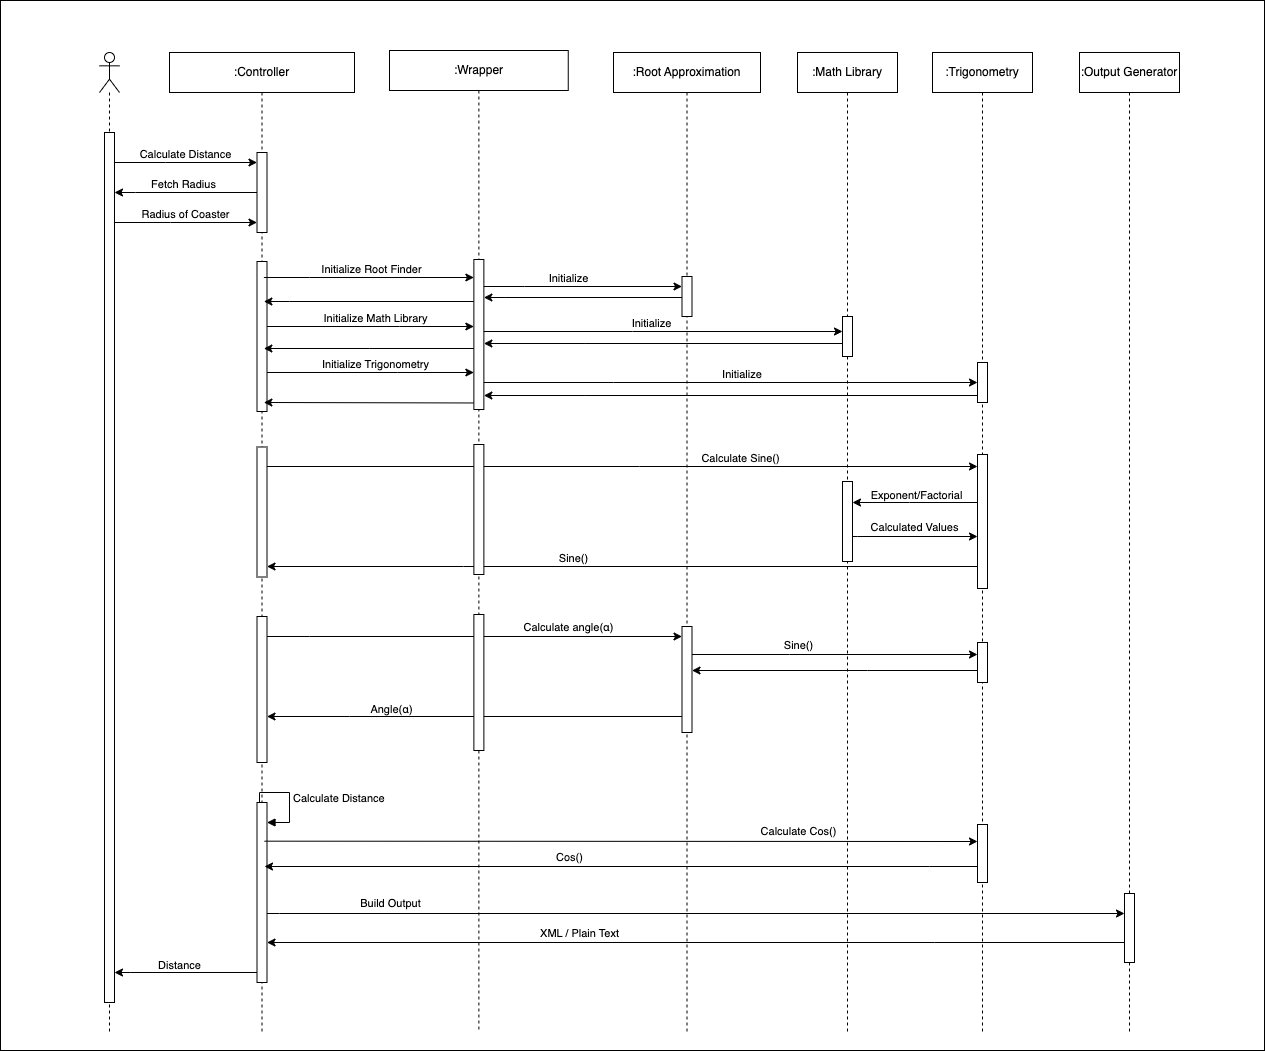
\includegraphics[width=1\linewidth]{resources/cheers-sequence.png}
        \vspace{.5cm}
        \caption{Flow of events for calculating the length}
        \label{fig:Sequence Diagram}
      \end{figure}
      \pagebreak

  \subsection{CRC Cards}
    \subsubsection{Trigonometry}
    \parbox{1.0\linewidth}{
      The trigonometry class is responsible for calculating the Sine and Cos of a given number. Its role is to calculate the Sin and Cos of a number using the McLaurin series to a pre-defined precision level. It collaborates with the Math Library class for accessing the exponent and factorial functions and with the Root Approximation class that need Sin and Cos for calculating the roots of the function.
    }
    \vspace*{2em}
    \begin{figure}[h!]
      \centering
      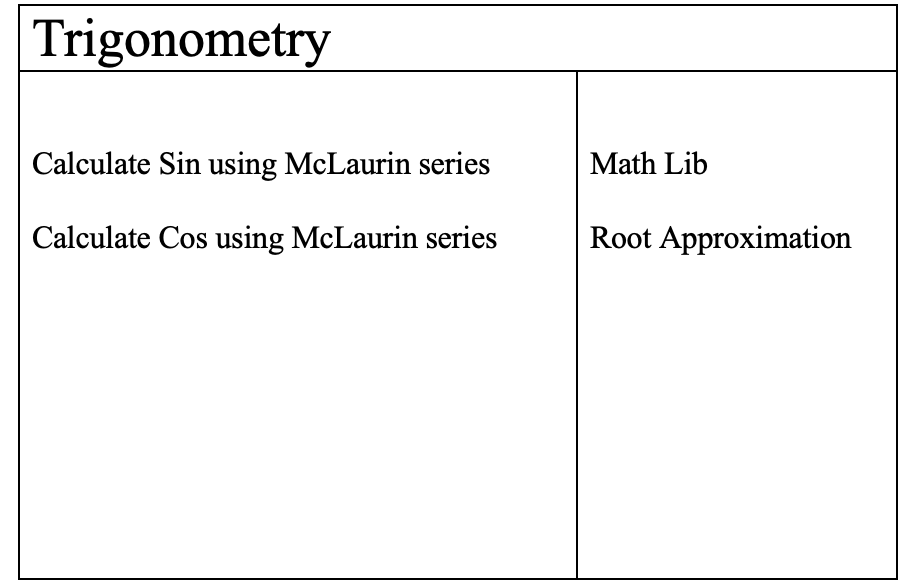
\includegraphics[width=.5\linewidth]{resources/Trigonometry.png}
      \caption{CRC Card - Trigonometry Class}\label{fig:trignometry}
    \end{figure} 

    \subsubsection{Math Library}
      \parbox{1.0\linewidth}{
        The responsibility of Math Lib class is to provide the function definition of Mathematical operations such as factorial and power of a given number. Its role is to calculate the value of PI using Leibniz formula, factorial and power of a given number using recursion. It collaborates with trigonometry, Root approximation and error handling class.
      }
      \vspace*{2em}
      \begin{figure}[h!]
        \centering
        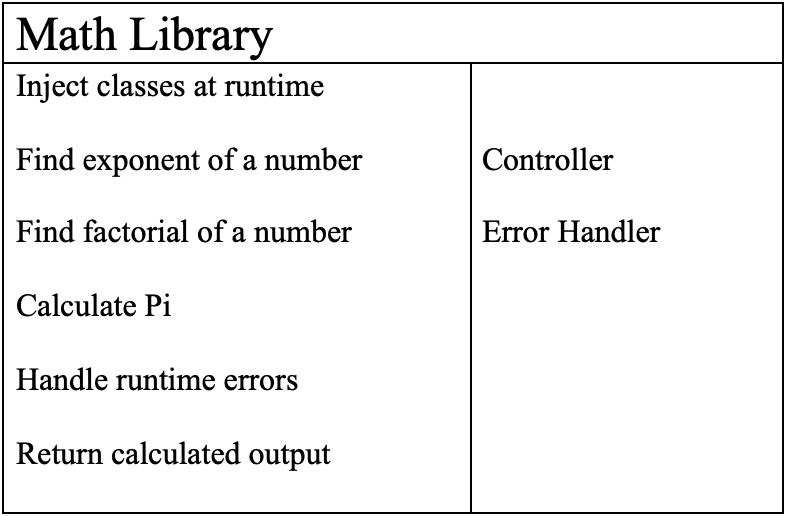
\includegraphics[width=.5\linewidth]{resources/MathLib.png}
        \caption{CRC Card - Math Library Class}\label{fig:mathlib}
      \end{figure}
      
    \subsubsection{Root Approximation}
      \parbox{1.0\linewidth}{
        The root approximation class is the core of the entire project. It contains two functions that calculate the roots of the given equation. It collaborates with Trigonometry and Math Lib classes as they contain necessary functions used for finding roots of an equation. As we always try to reduce the coupling with multiple classes and increase the cohesion within the class, we chose this class as to perform only one task of calculating the roots of equation.
      }
      \vspace*{2em}
      \begin{figure}[h!]
        \centering
        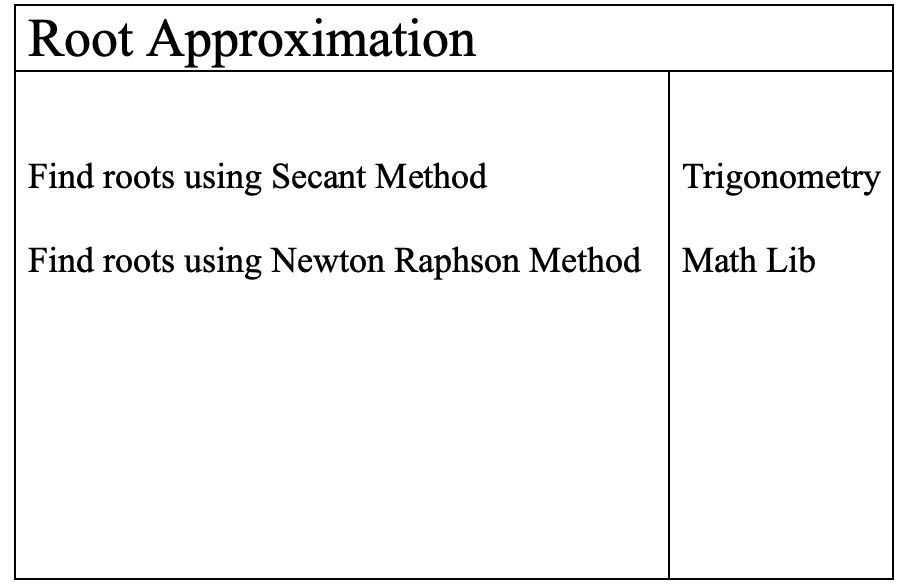
\includegraphics[width=.5\linewidth]{resources/RootApproximation.png}
        \caption{CRC Card - Root Approximation Class}\label{fig:rootapprox}
      \end{figure} 

    \subsubsection{Validator}
      \parbox{1.0\linewidth}{
        The role of the input validator class is to ensure that the data received from the user is in the appropriate format (positive integer). If the user enters invalid data, it prompts the user to provide valid data.
      }
      \vspace*{2em}
      \begin{figure}[h!]
        \centering
        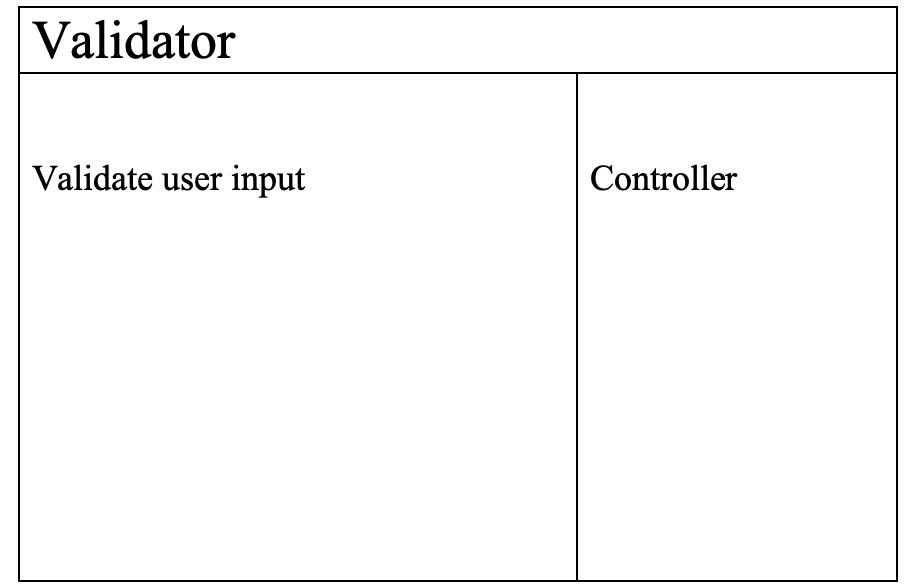
\includegraphics[width=.5\linewidth]{resources/Validator.png}
        \caption{CRC Card - Validator Class}\label{fig:validator}
      \end{figure}  

    \subsubsection{Error Handler}
      \parbox{1.0\linewidth}{
        The role of the error handler class is to handle errors that are generated. It collaborates with the controller class. The main responsibility of this class is to handle the errors generated and return an appropriate error message that is comprehensible to the user. The rationale for choosing this class is to define and handle all possible errors that are generated in the process of calculating length l.
      }
      \vspace*{2em}
      \begin{figure}[h!]
        \centering
        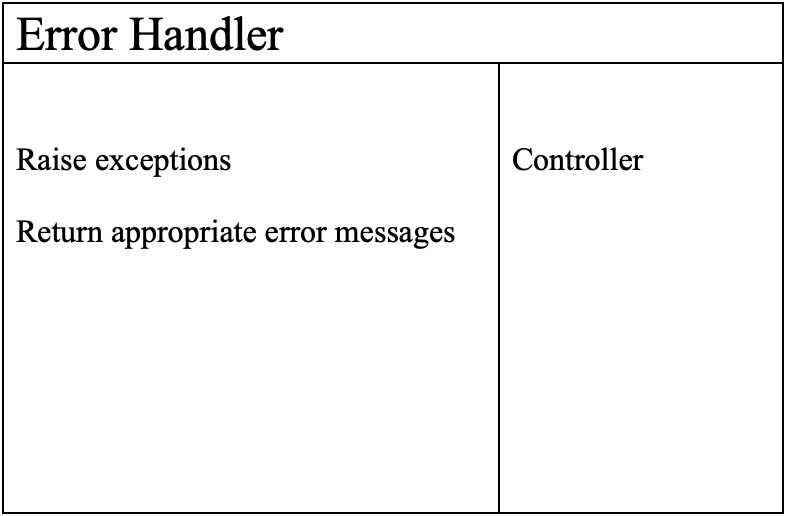
\includegraphics[width=.5\linewidth]{resources/ErrorHandler.png}
        \caption{CRC Card - Error Handler Class}\label{fig:error}
      \end{figure}

    \subsubsection{Output Generator}
      \parbox{1.0\linewidth}{
        The main role of the Output Generator class is to generate XML files. It stores the radius of the circle and the overlapping length l. The rationale behind choosing this class is to make sure that the processing and output are separated so that any changes to the output format do not affect the processing capabilities. This reduces the coupling between the classes.
      }
      \vspace*{2em}
      \begin{figure}[h!]
        \centering
        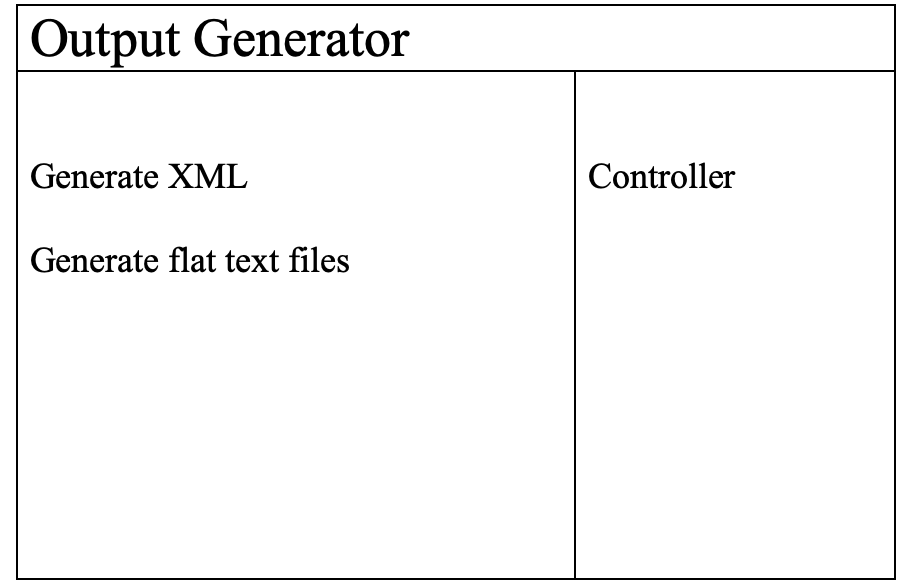
\includegraphics[width=.5\linewidth]{resources/OutputGenerator.png}
        \caption{CRC Card - OutputGenerator Class}\label{fig:output}
      \end{figure}

    \subsubsection{Controller}
      \parbox{1.0\linewidth}{
        The main role of this class is to calculate $\alpha$, the angle with a vertex at the centre of the left circle. It also calculates the length of the overlapping segment. To do this, it collaborates with other classes, which include Math Library, Trigonometry and Root Approximation. Each of these classes contains various mathematical functions such as Sine, Cos and Secant Approximation that are required for calculating the angle $\alpha$ and length l.
      }
      \vspace*{2em}
      \begin{figure}[h!]
        \centering
        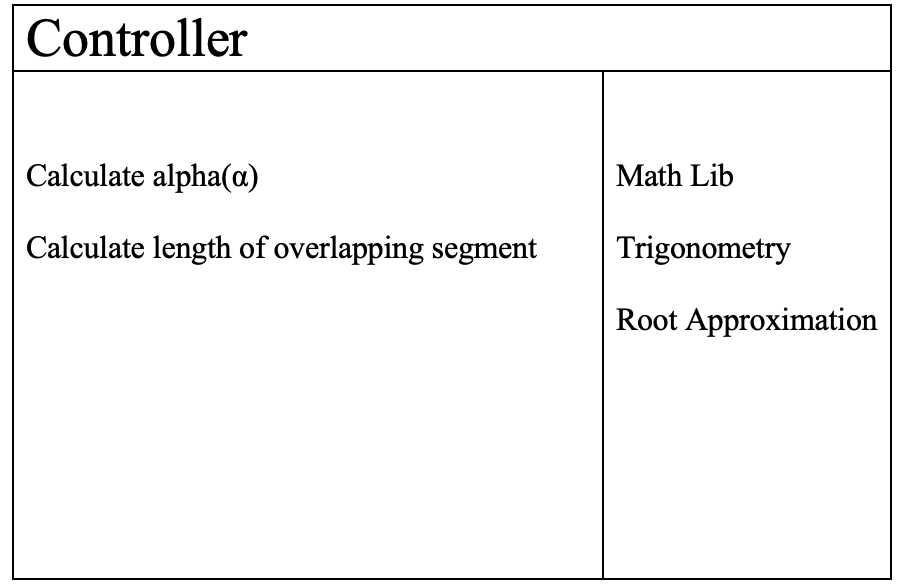
\includegraphics[width=.5\linewidth]{resources/Controller.png}
        \caption{CRC Card - Controller Class}\label{fig:control}
      \end{figure}

    \begin{figure}[h!]
      \centering
      \begin{tabular}{@{}c@{}}
        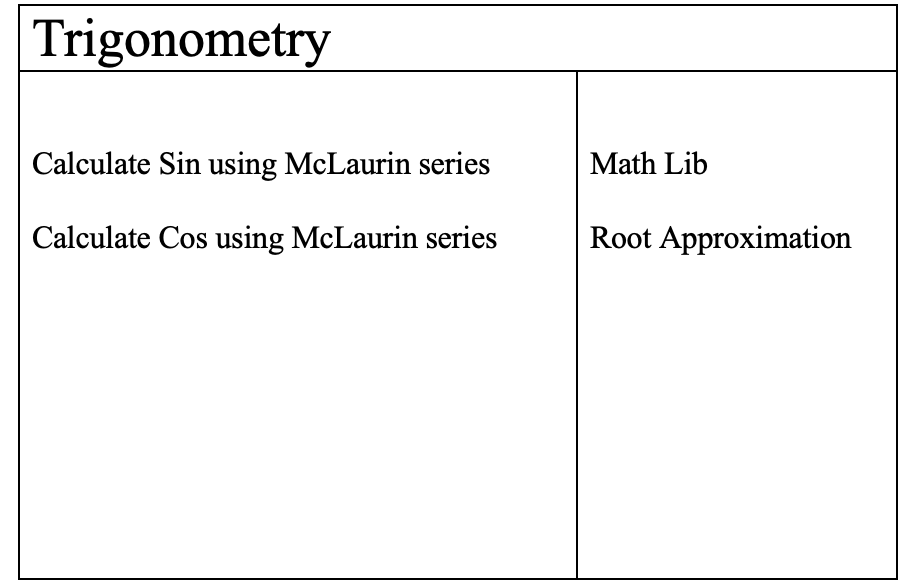
\includegraphics[width=.3\linewidth]{resources/Trigonometry.png} 
          \hspace*{30pt}
        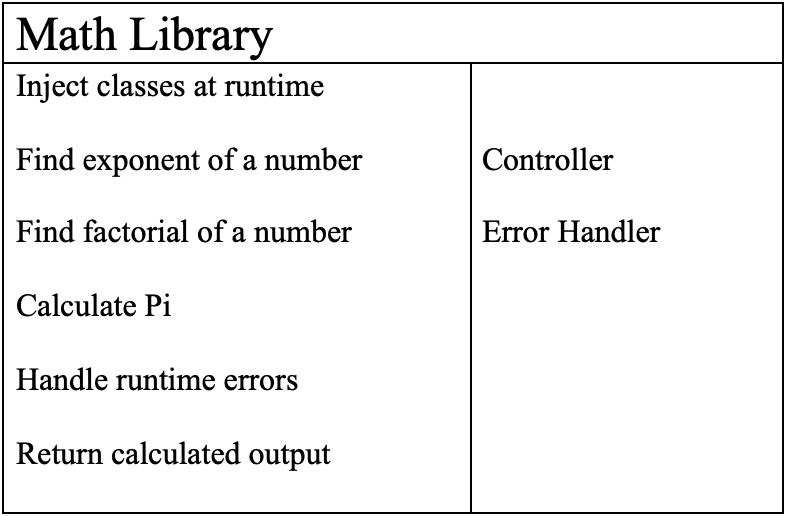
\includegraphics[width=.3\linewidth]{resources/MathLib.png}
      \end{tabular}
    
      \begin{tabular}{@{}c@{}}
          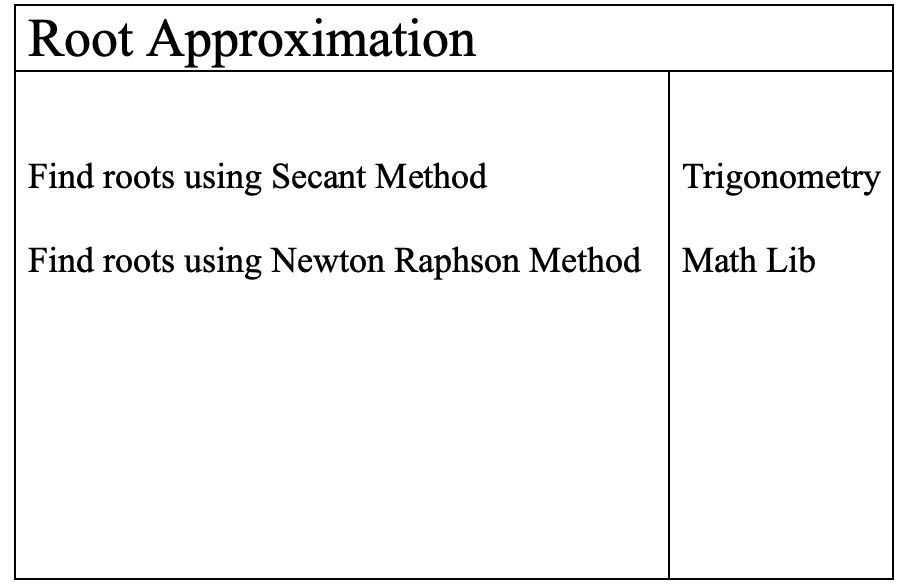
\includegraphics[width=.3\linewidth]{resources/RootApproximation.png} 
            \hspace*{30pt}
          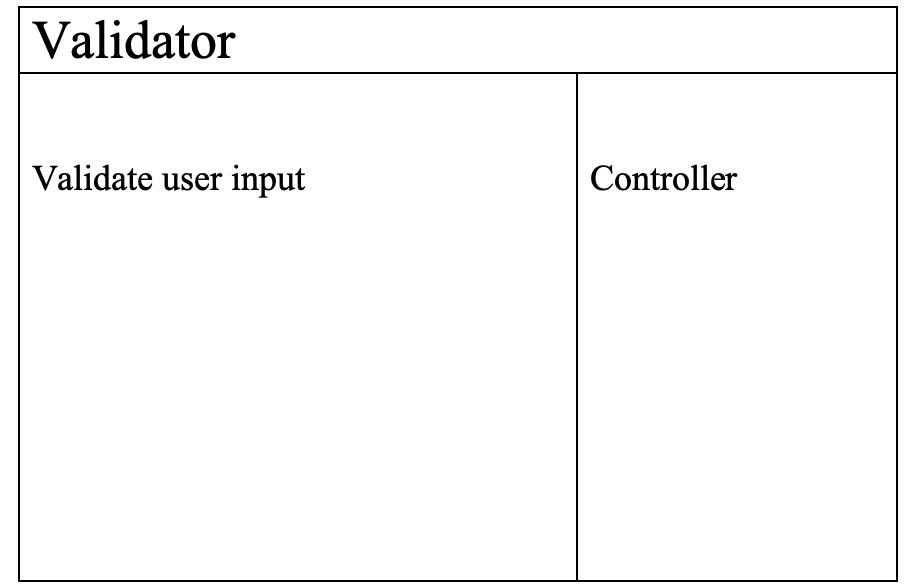
\includegraphics[width=.3\linewidth]{resources/Validator.png}
        \end{tabular}

        \begin{tabular}{@{}c@{}}
          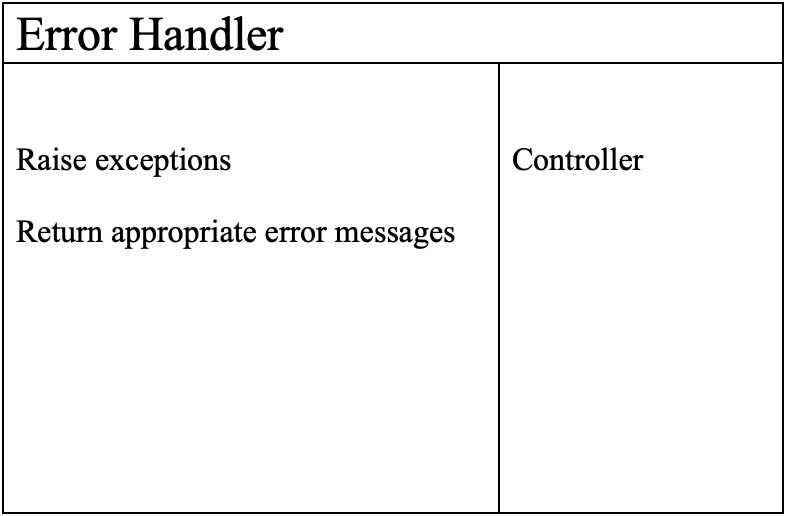
\includegraphics[width=.3\linewidth]{resources/ErrorHandler.png} 
            \hspace*{30pt}
          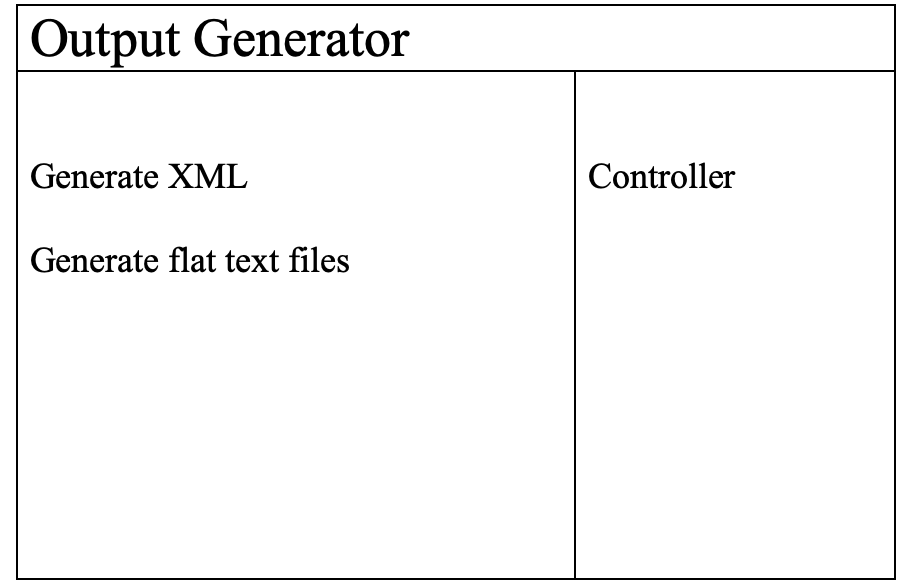
\includegraphics[width=.3\linewidth]{resources/OutputGenerator.png}
        \end{tabular}
        
        \begin{tabular}{@{}c@{}}
          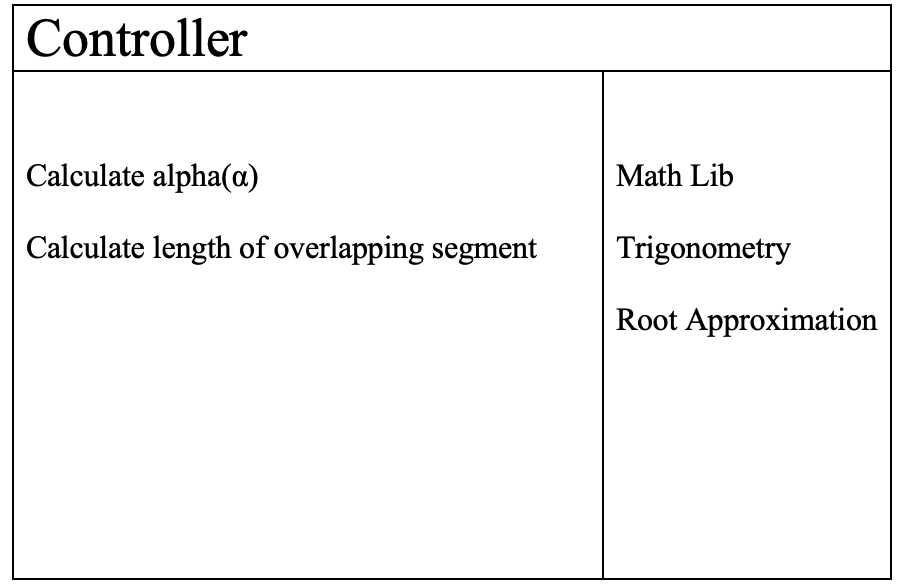
\includegraphics[width=.3\linewidth,height=90pt]{resources/Controller.png}
        \end{tabular}

        \vspace{\floatsep}
      \caption{Collection of CRC Cards for CHEERS}\label{fig:myfig}
    \end{figure}
